% !TEX root = saveliev_physics_general_course_2.tex
%!TEX TS-program = pdflatex
%!TEX encoding = UTF-8 Unicode


\chapter[ELASTIC WAVES]{ELASTIC WAVES}\label{chap:14}
\chaptermark{ELASTIC WAVES}

\section{Propagation of Waves in an Elastic Medium}\label{sec:14_1}

If at any place of an elastic (solid or fluid) medium its particles are made to oscillate, then owing to interaction between the particles, this oscillation will propagate in the medium from particle to particle with a certain velocity $v$.
The process of the propagation of oscillations in space is called a \textbf{wave}.

The particles of a medium in which a wave is propagating are not made to perform translational motion by the wave, they only oscillate about their equilibrium positions.
Depending on the direction of oscillations of particles relative to the direction of propagation of the wave, \textbf{longitudinal} and \textbf{transverse} waves are distinguished.
In the former, the particles of the medium oscillate along the direction of propagation of the wave.
In transverse waves, the particles of the medium oscillate in directions at right angles to the direction of wave propagation.
Elastic transverse waves can appear only in a medium having a resistance to shear.
Therefore, only longitudinal waves can appear in fluids.
Both longitudinal and transverse waves can appear in a solid.

Figure \ref{fig:14_1} shows the motion of the particles when a transverse wave propagates in a medium.
The numbers $1$, $2$, etc. designate particles spaced at a distance of $vT/4$, \ie, at the distance travelled by the wave during one-fourth of the period of the oscillations performed by the particles.
At the moment of time taken as zero, the wave propagating along the axis from left to right reached particle $1$.
As a result, the particle began to move upward from its equilibrium position, carrying the following particles along.
After one-fourth of a period, particle $1$ reaches its extreme top position; simultaneously, particle $2$ begins to move from its equilibrium position.
After another fourth of a period elapses, the first particle will pass its equilibrium position moving downward, the second particle will reach its extreme top position, and the third particle will begin to move upward from its equilibrium position.
At the moment $T$, the first particle will complete a cycle of oscillation and will be in the same state of motion as at the initial moment.
The wave by the moment $T$, having covered the path $vT$, will reach particle $5$.

\begin{figure}[t]
	\begin{center}
		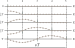
\includegraphics[scale=1]{figures/ch_14/fig_14_1.pdf}
		\caption[]{}
		\label{fig:14_1}
	\end{center}
	\vspace{-0.8cm}
\end{figure}

\begin{figure}[t]
	\begin{center}
		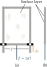
\includegraphics[scale=1]{figures/ch_14/fig_14_2.pdf}
		\caption[]{}
		\label{fig:14_2}
	\end{center}
	\vspace{-0.8cm}
\end{figure}

Figure \ref{fig:14_2} shows how the particles move when a longitudinal wave propagates in a medium.
All the reasoning relating to the behaviour of particles in a transverse wave can also be related to the given case with displacements to the right and left substituted for the upward and downward ones.
A glance at the figure shows that the propagation of a longitudinal wave in a medium is attended by alternating compensations and dilatations of the particles (the places of compensation of the particles are surrounded by a dash line in the figure).
They move in the direction of wave propagation with the velocity $v$.

Figures \ref{fig:14_1} and \ref{fig:14_2} show oscillations of particles whose equilibrium positions are on the $x$-axis.
Actually, not only the particles along the $x$-axis, but the entire collection of particles contained in a certain volume oscillate.
Spreading from the source of oscillations, the wave process involves new and new parts of space.
The locus of the points reached by the oscillations at the moment of time $t$ is called the \textbf{wavefront}.
The latter is the surface separating the part of space already involved in the wave process from the region in which oscillations have not yet appeared.

The locus of the points oscillating in the same phase is known as a \textbf{wave surface}.
A wave surface can be drawn through any point of the space involved in a wave process.
Hence, there is an infinitely great number of wave surfaces, whereas there is only one wavefront at each moment of time.
Wave surfaces remain stationary (they pass through the equilibrium positions of particles oscillating in the same phase).
A wavefront is in constant motion.

Wave surfaces can have any shape.
In the simplest cases, they are planes or spheres.
The wave in these cases is called plane or spherical,
accordingly.
In a plane wave, the wave surfaces are a multitude of parallel planes, in a spherical wave they are a multitude of concentric spheres.

Assume that a plane wave is propagating along the $x$-axis.
Hence, all the points of the medium whose equilibrium positions have an identical coordinate $x$ (but different values of $y$ and $z$) oscillate in the same phase.
Figure \ref{fig:14_3} shows a curve that produces the displacement $\xi$ of points having different $x$'s at a certain moment of time from their equilibrium position.
This figure must not be understood as a visible image of a wave.
It shows a graph of the function $\xi(x,t)$ for a certain fixed moment of time $t$.
Such a graph can be constructed for both a longitudinal and a transverse wave.

The distance $\lambda$ covered by a wave during the time equal to the period of oscillations of the particles of a medium is called the \textbf{wavelength}.
It is obvious that
\vspace{-12pt}
\begin{equation}\label{eq:14_1}
    \lambda = vT,
\end{equation}

\noindent
where $v$ is the velocity of the wave and $T$ is the period of oscillations.

\begin{figure}[t]
	\begin{center}
		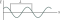
\includegraphics[scale=1]{figures/ch_14/fig_14_3.pdf}
		\caption[]{}
		\label{fig:14_3}
	\end{center}
	\vspace{-0.85cm}
\end{figure}

The wavelength can also be defined as the distance between the closest points of a medium that oscillate with a phase difference of $2\pi$ (see \fig{14_3}).

Substituting $1/\nu$ ($\nu$ is the frequency of oscillations) for $T$ in \eqn{14_1}, we get
\begin{equation}\label{eq:14_2}
    \lambda\nu = v.
\end{equation}

\noindent
We can also arrive at this equation from the following considerations.
In one second, a wave source completes $\nu$ oscillations, producing during each oscillation one ``crest'' and one ``trough'' in the medium.
By the moment when the source will complete its $\nu$-th oscillation, the first crest will cover the path $v$.
Consequently, the path $v$ must contain $\nu$ crests and troughs of the wave.

\section{Equations of a Plane and a Spherical Wave}\label{sec:14_2}

A wave equation is an expression that gives the displacement of an oscillating particle as a function of its coordinates $x$, $y$, $z$, and the time $t$:
\begin{equation}\label{eq:14_3}
    \xi = \xi(x,y,z,t)
\end{equation}

\noindent
(we have in mind the coordinates of the equilibrium position of the particle).
This function must be periodical both relative to the time t and to the coordinates $x$, $y$, $z$.
Its periodicity in time follows from the fact that $\xi$ describes the oscillations of a particle having the coordinates $x$, $y$, $z$.
Its periodicity with respect to the coordinates follows from the fact that points at a distance $\lambda$ from one another oscillate in the same way.

Let us find the form of the function $\xi$ for a plane wave assuming that the oscillations are harmonic.
For simplicity, we shall direct the coordinate axes so that the $x$-axis coincides with the direction of propagation of the wave.
The wave surfaces will therefore be perpendicular to the $x$-axis and, since all the points of the wave surface oscillate identically, the displacement $\xi$ will depend only on $x$ and on $t$, \ie, $\xi=\xi(x,t)$.
Let the oscillations of the points in the plane $x=0$ (\fig{14_4}) have the form
\begin{equation*}
    \xi(0,t) = A \cos(\omega t + \alpha).
\end{equation*}

\begin{figure}[t]
	\begin{center}
		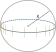
\includegraphics[scale=1]{figures/ch_14/fig_14_4.pdf}
		\caption[]{}
		\label{fig:14_4}
	\end{center}
	\vspace{-0.85cm}
\end{figure}

\noindent
Let us find the form of the oscillations of the points in the plane corresponding to an arbitrary value of $x$.
To travel the path from the plane $x=0$ to this plane, the wave needs the time $T=x/v$ (here, $v$ is the velocity of wave propagation).
Consequently, the oscillations of the particles in the plane $x$ will lag in time by $T$ behind the oscillations of the particles in the plane $x=0$, \ie, they will have the form
\begin{equation*}
    \xi(x,t) = A \cos[\omega(t - \tau) + \alpha] = A \cos\bracket{ \omega \parenthesis{t - \frac{x}{v}} + \alpha}.
\end{equation*}

Thus, the equation of a plane wave (both a longitudinal and a transverse one) propagating in the direction of the $x$-axis has the following form:
\begin{equation}\label{eq:14_4}
    \xi = A \cos\bracket{ \omega \parenthesis{t - \frac{x}{v}} + \alpha}.
\end{equation}

\noindent
The quantity $A$ is the amplitude of a wave.
The initial phase of the wave $\alpha$ is determined by our choice of the beginning of counting $x$ and $t$.
When considering one wave, the initial time and the coordinates are usually selected so that $\alpha$ is zero.
This cannot be done, as a rule, when considering several waves jointly.

Let us fix a value of the phase in \eqn{14_4} by assuming that
\begin{equation}\label{eq:14_5}
    \omega \parenthesis{t - \frac{x}{v}} + \alpha = \text{constant}.
\end{equation}

\noindent
This expression determines the relation between the time $t$ and the place $x$ where the phase has a fixed value.
The value of $\diffin{x}{t}$ ensuing from it gives the velocity with which the given value of the phase propagates.
Differentiation of \eqn{14_5} yields
\begin{equation*}
    \deriv{t} - \frac{1}{v}\, \deriv{x} = 0,
\end{equation*}

\noindent
whence
\begin{equation}\label{eq:14_6}
    \diff{x}{t} = v.
\end{equation}

\noindent
Thus, the velocity of wave propagation $v$ in \eqn{14_4} is the velocity of phase propagation, and in this connection it is called the \textbf{phase velocity}.

According to \eqn{14_6}, we have $\diffin{x}{t}>0$. Hence, \eqn{14_4} describes a wave propagating in the direction of growing $x$.
A wave propagating in the opposite direction is described by the equation
\begin{equation}\label{eq:14_7}
    \xi = A \cos\bracket{ \omega \parenthesis{t + \frac{x}{v}} + \alpha}.
\end{equation}

\noindent
Indeed, equating the phase of wave \eqref{eq:14_7} to a constant and differentiating the equation obtained, we arrive at the expression
\begin{equation*}
    \diff{x}{t} = -v,
\end{equation*}

\noindent
from which it follows that the wave given by \eqn{14_7} propagates in the direction of diminishing $x$.

The equation of a plane wave can be given a symmetrical form relative to $x$ and $t$.
For this purpose, let us introduce the quantity
\begin{equation}\label{eq:14_8}
    k = \frac{2\pi}{\lambda},
\end{equation}

\noindent
known as the \textbf{wave number}.
Multiplying the numerator and the denominator of \eqn{14_8} by the frequency $\nu$, we can represent the wave number in the form
\begin{equation}\label{eq:14_9}
    k = \frac{\omega}{\nu}
\end{equation}

\noindent
[see \eqn{14_2}].
Opening the parentheses in \eqn{14_4} and taking \eqn{14_9} into account, we arrive at the following equation for a plane wave propagating along the $x$-axis:
\begin{equation}\label{eq:14_10}
    \xi = A \cos(\omega t - kx + \alpha).
\end{equation}

\noindent
The equation of a wave propagating in the direction of diminishing $x$ differs from \eqn{14_10} only in the sign of the term $kx$.

In deriving \eqn{14_10}, we assumed that the amplitude of the oscillations does not depend on $x$.
This is observed for a plane wave when the energy of the wave is not absorbed by the medium.
When a wave propagates in a medium absorbing energy, the intensity of the wave gradually diminishes with an increasing distance from the source of oscillations---damping of the wave is observed.
Experiments show that in a homogeneous medium such damping occurs according to an exponential law: $A = A_0 e^{-\gamma x}$ [compare with the diminishing of the amplitude of damped oscillations with time; see Eq. (7.102) of Vol. I].
Accordingly, the equation of a plane wave has the following form:
\begin{equation}\label{eq:14_11}
    \xi = A_0\, e^{-\gamma x} \cos(\omega t - kx + \alpha)
\end{equation}

\noindent
($A_0$ is the amplitude at points in the plane $x=0$, and $\gamma$ is the attenuation coefficient).

Now, let us find the equation of a spherical wave.
Any real source of waves has a certain extent.
But if we limit ourselves to considering a wave at distances from its source appreciably exceeding the dimensions of the source, then the latter may be treated as a point one.
A wave emitted by a point source in an isotropic and homogeneous medium will be spherical.
Assume that the phase of oscillations of the source is $(\omega t + \alpha)$.
Hence, points on a wave surface of radius $r$ will oscillate with the phase $\omega (t - r/v) + \alpha = \omega_0t - kr + \alpha$ (the wave needs the time $\tau = r/v$ to travel the path $r$).
The amplitude of the oscillations in this case, even if the energy of the wave is not absorbed by the medium, does not remain constant---it diminishes with the distance from the source as $1/r$ (see \sect{14_6}).
Consequently, the equation of a spherical wave has the form
\begin{equation}\label{eq:14_12}
    \xi = \frac{A}{r} \cos(\omega t - kr + \alpha),
\end{equation}

\noindent
where $A$ is a constant quantity numerically equal to the amplitude at a distance of unity from the source.
The dimension of $A$ equals that of the oscillating quantity multiplied by the dimension of length.
The factor $e^{-\gamma r}$ must be multiplied to \eqn{14_12} for an absorbing medium.

We remind our reader that owing to the assumptions we have made, \eqn{14_12} holds only when $r$ appreciably exceeds the dimensions of the source. When $r$ tends to zero, the expression for the amplitude tends to infinity.
The explanation of this absurd result is that the equation cannot be used for small $r$'s.

\section{Equation of a Plane Wave Propagating in an Arbitrary Direction}\label{sec:14_3}

Let us find the equation of a plane wave propagating in a direction making the angles $\alpha$, $\beta$, $\gamma$ (not to be confused with the attenuation coefficient) with the coordinate axes $x$, $y$, $z$.
We shall assume that the oscillations in a plane passing through the origin of coordinates (\fig{14_5}) have the form
\begin{equation}\label{eq:14_13}
    \xi_0 = A \cos(\omega t + \alpha).
\end{equation}

\begin{figure}[t]
	\begin{center}
		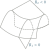
\includegraphics[scale=1]{figures/ch_14/fig_14_5.pdf}
		\caption[]{}
		\label{fig:14_5}
	\end{center}
	\vspace{-0.8cm}
\end{figure}

\noindent
Let us take a wave surface (plane) at the distance $l$ from the origin of coordinates.
The oscillations in this plane will lag behind those expressed by \eqn{14_13} by the time $\tau=l/v$:
\begin{equation}\label{eq:14_14}
    \xi = A \cos\bracket{ \omega \parenthesis{t - \frac{l}{v}} + \alpha} = A \cos(\omega t - kl + \alpha)
\end{equation}

\noindent
[$k = \omega/v$; see \eqn{14_9}].

Let us express $l$ through the position vector of points on the surface being considered.
For this purpose, we shall introduce the unit vector $\hatvec{n}$ of a normal to the wave surface.
A glance at \fig{14_5} shows that the scalar product of $\hatvec{n}$ and the position vector $\vec{r}$ of any point on the surface is $l$:
\begin{equation*}
    \hatvec{n} \ccdot \vec{r} = r\cos\varphi = l.
\end{equation*}

\noindent
Substitution of $\hatvec{n}\ccdot\vec{r}$ for l in \eqn{14_14} yields
\begin{equation}\label{eq:14_15}
    \xi = A \cos[\omega t - k (\hatvec{n}\ccdot\vec{r}) + \alpha].
\end{equation}

The vector
\begin{equation}\label{eq:14_16}
    \vec{k} = k \hatvec{n},
\end{equation}

\noindent
equal in magnitude to the wave number $k=2\pi/\lambda$ and directed along a normal to the wave surface is called the \textbf{wave vector}.
Thus, \eqn{14_15} can be written in the form
\begin{equation}\label{eq:14_17}
    \xi(\vec{r},t) = A \cos(\omega t - \vec{k} \ccdot \vec{r} + \alpha).
\end{equation}

\noindent
We have obtained the equation for a plane undamped wave propagating in the direction determined by the wave vector $\vec{k}$.
For a damped wave, the factor $e^{-\gamma l}=e^{-\gamma (\hatvec{n}\ccdot\vec{r})}$ must be added to the equation.

Function \eqref{eq:14_17} gives the deviation of a point having the position vector $\vec{r}$ from its equilibrium position at the moment of time $t$ (we remind our reader that $\vec{r}$ determines the equilibrium position of the point).
To pass over from the position vector of a point to its coordinates $x$, $y$, $z$, let us express the scalar product $\vec{k}\ccdot\vec{r}$ through the components of the vectors along the coordinate axes:
\begin{equation*}
    \vec{k}\ccdot\vec{r} = k_x x + k_y y + k_z z.
\end{equation*}

\noindent
The equation of a plane wave, therefore, becomes
\begin{equation}\label{eq:14_18}
    \xi(x,y,z; t) = A \cos\parenthesis{ \omega t - k_x x - k_y y - k_z z + \alpha}.
\end{equation}

\noindent
Here,
\begin{equation}\label{eq:14_19}
    k_x = \frac{2\pi}{\lambda}\cos\alpha,\quad k_y = \frac{2\pi}{\lambda}\cos\beta, \quad k_z = \frac{2\pi}{\lambda}\cos\gamma.
\end{equation}

\noindent
Function \eqref{eq:14_18} gives the deviation of a point having the coordinates $x$, $y$, $z$ at the moment of time $t$.
When $\hatvec{n}$ coincides with $\vecuni{x}$, we have $k_x = x$, $k_y = k_z = 0$, and \eqn{14_18} transforms into \eqn{14_10}.
It is very convenient to write the equation of a plane wave in the form
\begin{equation}\label{eq:14_20}
    \xi = \Re\bracket{ A e^{i(\omega t - \vec{k}\ccdot\vec{r} + \alpha)} }.
\end{equation}

\noindent
The symbol $\Re$ is usually omitted, having in mind that only the real part of the relevant expression is taken.
In addition, the complex number
\begin{equation}\label{eq:14_21}
    \hat{A} = A e^{i\alpha},
\end{equation}

\noindent
called the \textbf{complex amplitude} is introduced.
The magnitude of this number gives the amplitude, and the argument, the initial phase of the wave.

Thus, the equation of a plane undamped wave can be written in the form
\begin{equation}\label{eq:14_22}
    \xi = \hat{A} e^{i(\omega t - \vec{k}\ccdot\vec{r})}.
\end{equation}

\noindent
The advantages of writing the equation in this form will come to light later.

\section{The Wave Equation}\label{sec:14_4}

The equation of any wave is the solution of a differential equation called the \textbf{wave equation}.
To establish the form of the wave equation, let us compare the second partial derivatives with respect to the coordinates and time of function \eqref{eq:14_18} describing a plane wave.
Differentiating this function twice with respect to each of the variables, we get
\begin{align*}
    \diffnpartial{\xi}{t}{2} = -\omega^2 A \cos(\omega t - \vecdot{k}{r} + \alpha) = -\omega^2 \xi,\\
    \diffnpartial{\xi}{x}{2} = -k_x^2 A \cos(\omega t - \vecdot{k}{r} + \alpha) = -k_x^2 \xi,\\
    \diffnpartial{\xi}{y}{2} = -k_y^2 A \cos(\omega t - \vecdot{k}{r} + \alpha) = -k_y^2 \xi,\\
    \diffnpartial{\xi}{t}{2} = -k_z^2 A \cos(\omega t - \vecdot{k}{r} + \alpha) = -k_z^2 \xi.
\end{align*}

\noindent
Summation of the derivatives with respect to the coordinates yields
\begin{equation}\label{eq:14_23}
    \diffnpartial{\xi}{x}{2} + \diffnpartial{\xi}{y}{2} + \diffnpartial{\xi}{z}{2} = - (k_x^2 + k_y^2 + k_z^2) \xi = -k^2 \xi.
\end{equation}

\noindent
Comparing this sum with the time derivative and substituting $1/v^2$ for $k^2/\omega^2$ [see \eqn{14_9}], we get the equation
\begin{equation}\label{eq:14_24}
    \diffnpartial{\xi}{x}{2} + \diffnpartial{\xi}{y}{2} + \diffnpartial{\xi}{z}{2} = \frac{1}{v^2}\, \diffnpartial{\xi}{t}{2}.
\end{equation}

\noindent
This is exactly the wave equation.
It can be written in the form
\begin{equation}\label{eq:14:25}
    \upDelta{\xi} = \frac{1}{v^2}\, \diffnpartial{\xi}{t}{2},
\end{equation}

\noindent
where $\upDelta$ is the Laplacian operator [see \eqn{1_104}].

It is easy to convince ourselves that the wave equation is satisfied not only by function \eqref{eq:14_18}, but also by any function of the form
\begin{equation}\label{eq:14_26}
    f(x,y,z;t) = f(\omega t - k_x x - k_y y - k_z z + \alpha).
\end{equation}

\noindent
Indeed, denoting the expression in parentheses in the right-hand side of \eqn{14_26} by $\zeta$, we have
\begin{equation}\label{eq:14_27}
    \diffpartial{\zeta}{t} = \diffpartial{f}{\zeta} \diffpartial{\zeta}{t} = f' \omega,\quad \diffnpartial{f}{t}{2} = \omega \diffpartial{f'}{\zeta} \diffpartial{\zeta}{t} = \omega^2 f''.
\end{equation}

\noindent
Similarly,
\begin{equation}\label{eq:14_28}
    \diffnpartial{f}{x}{2} = k_x^2 f'',\quad \diffnpartial{f}{y}{2} = k_y^2 f'',\quad \diffnpartial{f}{z}{2} = k_z^2 f''.
\end{equation}

\noindent
Introducing \eqns{14_27}{14_28} into \eqn{14_24}, we arrive at the conclusion that function \eqref{eq:14_26} satisfies the wave equation if we assume that $v = \omega/k$.

Any function satisfying an equation of the form of \eqn{14_24} describes a wave; the square root of the quantity that is the reciprocal of the coefficient of $\diffnpartialin{\xi}{t}{2}$ gives the phase velocity of this wave.

We must note that for a plane wave propagating along the $x$-axis, the wave equation has the form
\begin{equation}\label{eq:14_29}
    \diffnpartial{\xi}{x}{2} = \frac{1}{v^2} \diffnpartial{\xi}{t}{2}.
\end{equation}

\section{Velocity of Elastic Waves in a Solid Medium}\label{sec:14_5}

\begin{figure}[t]
	\begin{center}
		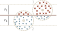
\includegraphics[scale=1]{figures/ch_14/fig_14_6.pdf}
		\caption[]{}
		\label{fig:14_6}
	\end{center}
	\vspace{-0.8cm}
\end{figure}

Assume that a longitudinal plane wave propagates in the direction of the $x$-axis.
Let us separate in the medium a cylindrical volume with a base area of $S$ and a height of $\Delta{x}$ (\fig{14_6}).
The displacements s of particles with different $x$'s are different at each moment of time (see \fig{14_3} showing $\xi$ against $x$).
If the base of the cylinder with the coordinate $x$ has at a certain moment of time the displacement $\xi$, then the displacement of a base with the coordinate $x+\Delta{x}$ will be $\xi+\Delta{\xi}$.
Therefore, the volume being considered will be deformed---it receives the elongation $\Delta{\xi}$ ($\Delta{\xi}$ is an algebraic quantity, $\Delta{\xi}<0$ corresponds to compression of the cylinder) or the relative elongation $\Delta{\xi}/\Delta{x}$.
The quantity $\Delta{\xi}/\Delta{x}$ gives the average deformation of the cylinder.
Since $\xi$ varies with $x$ according to a non-linear law, the true deformation in different cross sections of the cylinder will differ.
To obtain the deformation (strain) in the cross section $x$, we must make $\Delta{x}$ tend to zero.
Thus,
\begin{equation}\label{eq:14_30}
	\varepsilon = \diffpartial{\xi}{x}
\end{equation}

\noindent
(we have used the symbol of the partial derivative because $\xi$ depends not only on $x$, but also on $t$).

The presence of tensile strain points to the existence of the normal stress $\sigma$ which at small strains is proportional to the strain. According to Eq. (2.30) of Vol. I,
\begin{equation}\label{eq:14_31}
	\sigma = E \varepsilon = E = \diffpartial{\xi}{x}
\end{equation}

\noindent
($E$ is Young's modulus of the medium).
We must note that the unit strain $\diffpartialin{\xi}{x}$ and, consequently, the stress $\sigma$ at a fixed moment of time depend on $x$ (\fig{14_7}).
Where the deviations of the particles from their equilibrium position are maximum, the strain and the stress are zero.
Where the particles are passing through their equilibrium position, the strain and stress reach their maximum values, the positive and negative strains (\ie, tensions and compressions) alternating.
Accordingly, as we have already noted in \sect{14_1}, a longitudinal wave consists of alternating compressions and dilatations of the medium.

\begin{figure}[t]
	\begin{center}
		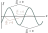
\includegraphics[scale=1.1]{figures/ch_14/fig_14_7.pdf}
		\caption[]{}
		\label{fig:14_7}
	\end{center}
	\vspace{-0.8cm}
\end{figure}

Let us revert to the cylindrical volume depicted in \fig{14_6} and write an equation of motion for it.
Assuming that $\Delta{x}$ is very small, we can consider that the projection of the acceleration onto
the $x$-axis is the same for all points of the cylinder and is $\diffpartialin{\xi}{x}$.
The mass of the cylinder is $\rho S\Delta{x}$, where $\rho$ is the density of the undeformed medium.
The projection onto the $x$-axis of the force acting on the cylinder equals the product of the area $S$ of the cylinder base and the difference between the normal stresses in the cross sections $(x+\Delta{x} +\xi + \Delta{\xi})$ and $(x+\xi)$:
\begin{equation}\label{eq:14_32}
	F_x = SE \bracket{ \parenthesis{ \diffpartial{\xi}{x} }_{x + \Delta{x} +\xi + \Delta{\xi}} - \parenthesis{ \diffpartial{\xi}{x} }_{x + \xi} }.
\end{equation}

The value of the derivative $\diffpartialin{\xi}{x}$ in the section $X + \delta$ can be written with great accuracy for small values of $\delta$ in the form
\begin{equation}\label{eq:14_33}
	\parenthesis{ \diffpartial{\xi}{x} }_{x+\delta} = \parenthesis{ \diffpartial{\xi}{x} }_{x} + \bracket{ \diffpartial{}{x} \parenthesis{ \diffpartial{\xi}{x} } }_x\, \delta = \parenthesis{ \diffpartial{\xi}{x} }_{x} + \diffnpartial{\xi}{x}{2}\, \delta,
\end{equation}

\noindent
where by $\diffnpartialin{\xi}{x}{2}$ is meant the value of the second partial derivative of $\xi$ with respect to $x$ in the cross section $x$.

Owing to the smallness of the quantities $\Delta{x}$, $S$, and $\Delta{\xi}$, we can perform transformation \eqref{eq:14_33} in \eqn{14_32}:
\begin{align}
	F_x &= SE \bracet{
	\bracket{
	\parenthesis{ \diffpartial{\xi}{x} }_{x}  + \diffnpartial{\xi}{x}{2} (\Delta{x}+\xi+\Delta{\xi})
	} -
	\bracket{
	\parenthesis{ \diffpartial{\xi}{x} }_{x} + \diffnpartial{\xi}{x}{2} \xi
	}
	}\nonumber\\
	&= SE \diffnpartial{\xi}{x}{2} (\Delta{x} + \Delta{\xi}) \approx SE \diffnpartial{\xi}{x}{2} \Delta{x} \label{eq:14_34}
\end{align}

\noindent
[the relative elongation $\diffpartialin{\xi}{x}$ in elastic deformations is much smaller than unity.
Consequently, $\Delta{\xi}\ll\Delta{x}$ so that the addend $\Delta{\xi}$ in the sum $(\Delta{x} + \Delta{\xi})$ may be disregarded].

Introducing the found values of the mass, acceleration, and force into the equation of Newton's second law, we get
\begin{equation*}
	\rho S \Delta{x} \diffnpartial{\xi}{t}{2} = SE \diffnpartial{\xi}{x}{2} \Delta{x}.
\end{equation*}

\noindent
Finally, cancelling $S\Delta{x}$, we arrive at the equation
\begin{equation}\label{eq:14_35}
	\diffnpartial{\xi}{x}{2} = \frac{\rho}{E} \diffnpartial{\xi}{t}{2},
\end{equation}

\noindent
which is the wave equation for the case when $\xi$ is independent of $y$ and $z$.
A comparison of \eqns{14_29}{14_35} shows that
\begin{equation}\label{eq:14_36}
	v = \parenthesis{\frac{E}{\rho}}^{1/2},
\end{equation}

\noindent
Thus, the phase velocity of longitudinal elastic waves equals the square root of Young's modulus divided by the density of the medium.

Similar calculations for transverse waves lead to the expression
\begin{equation}\label{eq:14_37}
	v = \parenthesis{\frac{G}{\rho}}^{1/2},
\end{equation}

\noindent
where $G$ is the shear modulus.

\section{Energy of an Elastic Wave}\label{sec:14_6}

Assume that the plane longitudinal wave,
\begin{equation*}
	\xi = A \cos(\omega t - kx + \alpha)
\end{equation*}

\noindent
[see \eqn{14_10}], is propagating in the direction of the $x$-axis in a certain medium.
Let us separate in this medium an elementary volume $\Delta{V}$ so small that the velocity and the strain at all the points of this volume may be considered the same and equal, respectively, to $\diffpartialin{\xi}{t}$ and $\diffpartialin{\xi}{x}$.

The volume we have separated has the kinetic energy
\begin{equation}\label{eq:14_38}
	\ab{\Delta{W}}{k} = \frac{\rho}{2} \parenthesis{\diffpartial{\xi}{t}}^2 \Delta{V}
\end{equation}

\noindent
($\rho\Delta{V}$ is the mass of the volume, and $\diffpartialin{\xi}{t}$ is its velocity).

According to Eq. (3.81) of Vol. I, the volume being considered also has the potential energy of elastic deformation
\begin{equation*}
	\ab{\Delta{W}}{p} = \frac{E\varepsilon^2}{2} \Delta{V}  = \frac{E}{2} \parenthesis{\diffpartial{\xi}{x}}^2 \Delta{V}
\end{equation*}

\noindent
($\varepsilon=\diffpartialin{\xi}{x}$ is the relative elongation of the cylinder, $E$ is Young's
modulus of the medium).
Let us use \eqn{14_36} to substitute $\rho v^2$ for Young's modulus ($\rho$ is the density of the medium, and $v$ is the phase velocity of the wave).
Hence, the expression for the potential energy of the volume $\Delta{V}$ acquires the form
\begin{equation}\label{eq:14_39}
	\ab{\Delta{W}}{p} = \frac{E\varepsilon^2}{2} \parenthesis{\diffpartial{\xi}{x}}^2 \Delta{V}.
\end{equation}

The sum of \eqns{14_38}{14_39} gives the total energy
\begin{equation}\label{eq:14_40}
	\Delta{W} = \ab{\Delta{W}}{k} + \ab{\Delta{W}}{p} = \frac{1}{2} \rho \bracket{ \parenthesis{\diffpartial{\xi}{t}}^2 + v^2 \parenthesis{\diffpartial{\xi}{x}}^2 } \Delta{V}.
\end{equation}

\noindent
Dividing this energy by the volume $\Delta{V}$ in which it is contained, we get the energy density
\begin{equation}\label{eq:14_41}
	w = \frac{1}{2} \rho \bracket{ \parenthesis{\diffpartial{\xi}{t}}^2 + v^2 \parenthesis{\diffpartial{\xi}{x}}^2 }.
\end{equation}

Differentiation of \eqn{14_10} once with respect to $t$ and another time with respect to $x$ yields:
\begin{align*}
	\diffpartial{\xi}{t} &= - A\omega \sin(\omega t - kx + \alpha),\\
	\diffpartial{\xi}{x} &=  kA \sin(\omega t - kx + \alpha).
\end{align*}

\noindent
Introducing these equations into \eqn{14_41} and taking into account that $k^2v^2=\omega^2$, we get
\begin{equation}\label{eq:14_42}
	w = \rho A^2 \omega^2 \sin^2(\omega t - kx + \alpha).
\end{equation}

\noindent
A similar expression for the energy density is obtained for a transverse wave.

It can be seen from \eqn{14_42} that the energy density at each moment of time is different at different points of space.
At the same point, the energy density varies with time as the square of the sine.
The average value of sine square is one-half. Accordingly, the time-averaged value of the energy density at each point of a medium is
\begin{equation}\label{eq:14_43}
	\average{w} = \frac{1}{2} \rho A^2 \omega^2.
\end{equation}

\noindent
The energy density given by \eqn{14_42} and its average value [\eqn{14_43}] are proportional to the density of the medium $\rho$, the square of the frequency $\omega$, and the square of the wave amplitude $A$.
Such a relation holds not only for an undamped plane wave, but also for other kinds of waves (a plane damped wave, a spherical wave, etc.).

Thus, a medium in which a wave is propagating has an additional store of energy.
The latter is supplied to the different points of the medium from the source of oscillations by the wave itself; consequently, a wave carries energy with it.
The amount of energy carried by a wave through a surface in unit time is called the \textbf{energy ftux} through this surface.
If the energy $\deriv{W}$ is carried through a given
surface during the time $\deriv{t}$, then the energy flux $\Phi$ is
\begin{equation}\label{eq:14_44}
	\Phi = \diff{W}{t}.
\end{equation}

\noindent
The energy flux is a scalar quantity whose dimension equals that of energy divided by the dimension of time, \ie, coincides with the dimension of power.
Accordingly, $\Phi$ is measured in watts, \si{\erg\per\second}, etc.

The energy flux at different points of a medium can have a different intensity.
To characterize the flow of energy at different points of space, a vector quantity called the \textbf{density of the energy flux} is introduced.
It numerically equals the energy flux through a unit area placed at the given point perpendicular to the direction in which the energy is being transferred.
The direction of the vector of the energy flux density coincides with that of energy transfer.

Assume that the energy $\deriv{W}$ is transferred during the time $\deriv{t}$ through the area $\Delta{S}_{\perp}$ perpendicular to the direction of propagation of a wave.
The energy flux density will therefore be
\begin{equation}\label{eq:14_45}
	j = \frac{\Delta{\Phi}}{\Delta{S}_{\perp}} = \frac{\Delta{W}}{\Delta{S}_{\perp} \Delta{t}}
\end{equation}

\begin{figure}[t]
	\begin{center}
		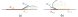
\includegraphics[scale=1]{figures/ch_14/fig_14_8.pdf}
		\caption[]{}
		\label{fig:14_8}
	\end{center}
	\vspace{-0.9cm}
\end{figure}

\noindent
[see \eqn{14_44}].
The energy $\Delta{W}$ confined in a cylinder with the base $\Delta{S}_{\perp}$ and the altitude $v\Delta{t}$ ($v$ is the phase velocity of the wave) will be transferred through the area $\Delta{S}_{\perp}$ (\fig{14_8}) during the time $\Delta{t}$.
If the dimensions of the cylinder are sufficiently small (as a result of the smallness of $\Delta{S}_{\perp}$ and $\Delta{t}$) to consider that the energy density at all points of the cylinder is the same, then $\Delta{W}$ can be found as the product of the energy density $w$ and the volume of the cylinder equal to $\Delta{S}_{\perp}v\Delta{t}$:
\begin{equation*}
	\Delta{W} = w \Delta{S}_{\perp} v \Delta{t}.
\end{equation*}

\noindent
Using this expression in \eqn{14_45}, we get the following equation for the density of the energy:
\begin{equation}\label{eq:14_46}
	j = wv.
\end{equation}

\noindent
Finally, introducing the vector $\vec{v}$ whose magnitude equals the phase velocity of the wave and whose direction coincides with that of wave propagation (and energy transfer), we can write
\begin{equation}\label{eq:14_47}
	\vec{j} = w \vec{v}.
\end{equation}

We have obtained an expression for the vector of the energy flux density.
This vector was first introduced by the outstanding Russian physicist Nikolai Umov (1846-1915) and is called \textbf{Umov's vector}.

The vector given by \eqn{14_47}, like the energy density $w$, is different at different points of space.
At a given point, it varies in time according to a sine square law.
Its average value is
\begin{equation}\label{eq:14_48}
	\average{\vec{j}} = \average{w} \vec{v} = \frac{1}{2} \rho A^2 \omega^2 \vec{v}
\end{equation}

\noindent
[see \eqn{14_43}].
Equation \eqref{eq:14_48}, like \eqn{14_43}, holds for a wave of any kind (spherical, damped, etc.).
We shall note that when we speak of the intensity of a wave at a given point, we have in mind the time-averaged value of the density of the energy flux transferred by the wave.

Knowing $\vec{j}$ for all the points of an arbitrary
surface $S$, we can calculate the energy flux through this surface.
For this purpose, let us divide the surface into elementary areas $\deriv{S}$.
During the time $\deriv{t}$, the energy $\deriv{W}$ confined in the oblique cylinder shown in \fig{14_9} will pass through area $\deriv{S}$.
The volume of this cylinder is $\deriv{V} = v\, \deriv{t}\, \deriv{S}\, \cos\varphi$.
It contains the energy $\deriv{W} = w\, \deriv{V} = wv\, \deriv{t}\, \deriv{S}\, \cos\varphi$ (here, $w$ is the instantaneous value of the energy density where area $\deriv{S}$ is).
Taking into account that
\begin{equation*}
	wv\, \deriv{S}\, \cos\varphi = j\, \deriv{S}\, \cos\varphi = \vec{j} \ccdot \derivec{S}
\end{equation*}

\noindent
($\derivec{S}=\hatvec{n}\,\deriv{S}$; see \fig{14_9}), we can write: $\deriv{W} = \vec{j} \ccdot \derivec{S}\, \deriv{t}$.
Hence, we obtain the following equation for the energy flux $\deriv{\Phi}$ through area $\deriv{S}$:
\begin{equation}\label{eq:14_49}
	\deriv{\Phi} = \diff{W}{t} = \vec{j} \ccdot \derivec{S}
\end{equation}

\begin{figure}[t]
	\begin{center}
		
\includegraphics[scale=0.95]{figures/ch_14/fig_14_9.pdf}
		\caption[]{}
		\label{fig:14_9}
	\end{center}
	\vspace{-0.9cm}
\end{figure}

\noindent
[compare with \eqn{1_72}].
The total energy flux through a surface equals the sum of the elementary fluxes given by \eqn{14_49}:
\begin{equation}\label{eq:14_50}
	\Phi = \int_S \vec{j} \ccdot \derivec{S}.
\end{equation}

\noindent
We can say in accordance with \eqn{1_74} that the energy flux equals the flux of the vector $\vec{j}$ through surface $S$.

Substituting for the vector $\vec{j}$ in \eqn{14_50} its time-averaged value, we get the average value of $\Phi$:
\begin{equation}\label{eq:14_51}
	\average{\Phi} = \int_S \average{\vec{j}} \ccdot \derivec{S}.
\end{equation}

Let us calculate the mean value of the energy flux through an arbitrary wave surface of an undamped spherical wave.
At each point of this surface, the vectors $\vec{j}$ and $\derivec{S}$ coincide in direction.
In addition, the magnitude of the vector $\vec{j}$ for all points of the surface is identical.
Hence,
\begin{equation*}
	\average{\Phi} = \int_S \average{j}\, \deriv{S} = \average{j} S = \average{j} 4\pi r^2
\end{equation*}

\noindent
($r$ is the radius of the wave surface).
According to \eqn{14_48}, we have $\average{j}=\rho A^2\omega^2v/2$.
Thus,
\begin{equation*}
	\average{\Phi} = 2\pi \rho \omega^2 A_r^2 r^2
\end{equation*}

\noindent
($A_r$ is the amplitude of the wave at a distance $r$ from its source).
Since the energy of the wave is not absorbed by the medium, the average energy flux through a sphere of any radius must have the same value, \ie, the condition
\begin{equation*}
	A_r^2 r^2 = \text{constant}
\end{equation*}

\noindent
must be observed.
It follows that the amplitude $A_r$ of an undamped spherical wave is inversely proportional to the distance $r$ from the wave source [see \eqn{14_12}].
Accordingly, the mean density of the energy flux $\average{j}$ is inversely proportional to the square of the distance from the source.

For a plane damped wave, the amplitude diminishes with the distance according to the law $A = A_0\,e^{-\gamma x}$ [see \eqn{14_11}].
The average density of the energy flux (\ie, the wave intensity) correspondingly diminishes according to the law
\begin{equation}\label{eq:14_52}
	j = j_0\, e^{-\varkappa x}.
\end{equation}

\noindent
Here, $\varkappa = 2\gamma$ is a quantity called the \textbf{wave absorption coefficient}.
Its dimension is the reciprocal of that of length.
It is easy to see that the reciprocal of $\varkappa$ equals the distance over which the intensity of a wave diminishes to $1/e$ of its initial value.

\section{Standing Waves}\label{sec:14_7}

If several waves propagate in a medium simultaneously, then the oscillations of the particles of the medium will be the geometrical sum of the oscillations which the particles would perform if each of the waves propagated separately.
Hence, the waves are simply superposed onto one another without disturbing one another.
This statement following from experiments is called the \textbf{principle of superposition of waves}.

When the oscillations due to separate waves at each point of a medium have a constant phase difference, the waves are called \textbf{coherent}.
(A stricter definition of coherence will be given in \sect{17_2}).
The summation of coherent waves gives rise to the phenomenon of \textbf{interference}, consisting in that the oscillations at some points amplify, and at other points weaken one another.

A very important case of interference is observed in the superposition of two plane waves having the same amplitude and approaching each other from opposite directions.
The resulting oscillatory process is called a \textbf{standing wave}.
Standing waves are produced when waves are reflected from obstacles.
The wave striking an obstacle and the reflected wave travelling toward it in the opposite direction as a result of superposition produce a standing wave.

Let us write the equations of two plane waves propagating along the $x$-axis in opposite directions:
\begin{align*}
	\xi_1 = A \cos(\omega t - kx + \alpha_1),\\
	\xi_2 = A \cos(\omega t + kx + \alpha_2).
\end{align*}

\noindent
Adding these two equations and transforming the result according to the formula for the sum of cosines, we get
\begin{equation}\label{eq:14_53}
	\xi = \xi_1 + \xi_2 = 2A \cos\bracket{kx + \parenthesis{\frac{\alpha_2-\alpha_1}{2}}} \cos\bracket{\omega t + \parenthesis{\frac{\alpha_1+\alpha_2}{2}}}.
\end{equation}

\noindent
Equation \eqref{eq:14_53} is the equation of a standing wave.
To simplify it, let us choose the beginning of reading $x$ so that the difference $\alpha_2-\alpha_1$ vanishes, and the beginning of reading $t$ so that the sum $\alpha_1+\alpha_2$ vanishes.
We shall also substitute for the wave number $k$ its value $2\pi/\lambda$.
Equation \eqref{eq:14_53} now becomes
\begin{equation}\label{eq:14_54}
	\xi = \bracket{2 A \cos\parenthesis{\frac{2\pi x}{\lambda}}} \cos(\omega t).
\end{equation}

A glance at \eqn{14_54} shows that at every point of a standing wave the oscillations have the same frequency as those of the opposite waves, the amplitude depending on $x$:
\begin{equation*}
	\text{amplitude} = \absolute{2 A \cos\parenthesis{\frac{2\pi x}{\lambda}}}.
\end{equation*}

\noindent
At the points whose coordinates comply with the condition
\begin{equation}\label{eq:14_55}
	\frac{2\pi x}{\lambda} = \pm n \pi\quad (n = 0, 1, 2, \ldots),
\end{equation}

\noindent
the amplitude of the oscillations reaches its maximum value.
These points are known as \textbf{antinodes} of the standing wave.
We obtain the values of the antinode coordinates from \eqn{14_55}:
\begin{equation}\label{eq:14_56}
	\ab{x}{anti} = \pm n \frac{\lambda}{2}\quad (n = 0, 1, 2, \ldots).
\end{equation}

It must be borne in mind that an antinode is not a single point, but a plane whose points have the value of the coordinate $x$ determined by \eqn{14_56}.

At the points whose coordinates comply with the condition
\begin{equation*}
	\frac{2\pi x}{\lambda} = \pm \parenthesis{n + \frac{1}{2}} \pi \quad (n = 0, 1, 2, \ldots),
\end{equation*}

\noindent
the amplitude of the oscillations vanishes.
These points are called the \textbf{nodes} of the standing wave.
The points of the medium at the nodes do not oscillate.
The coordinates of the nodes have the values
\begin{equation}\label{eq:14_57}
	\ab{x}{node} = \pm \parenthesis{n + \frac{1}{2}} \frac{\lambda}{2} \quad (n = 0, 1, 2, \ldots).
\end{equation}

\noindent
A node, like an antinode, is not a single point, but a plane whose points have values of the coordinate $x$ determined by \eqn{14_57}.

Examination of \eqns{14_56}{14_57} shows that the distance between adjacent antinodes, like that between adjacent nodes, is $\lambda/2$.
The antinodes and nodes are displaced relative to one another by a quarter of a wavelength.

Let us revert to \eqn{14_54}.
The factor $2A\cos(2\pi x/\lambda)$ changes its sign after passing through its zero value.
Accordingly, the phase of the oscillations at different sides of a node differs by $n$.
This signifies that points at different sides of a node oscillate in counterphase.
All the points between two adjacent nodes oscillate in phase.
Figure \ref{fig:14_10} contains a number of ``instantaneous photographs'' of the deviations of the points from their equilibrium position.
The first of them corresponds to the moment when the deviations reach their greatest absolute value.
The following ``photographs'' have been made at intervals of one-fourth of a period.
The arrows show the velocities of the particles.

% \begin{figure}[t]
% 	\begin{center}
% 		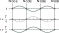
\includegraphics[scale=1]{figures/ch_14/fig_14_10.pdf}
% 		\caption[]{}
% 		\label{fig:14_10}
% 	\end{center}
% 	\vspace{-0.8cm}
% \end{figure}
\begin{figure}[t]
	\begin{minipage}[t]{0.48\linewidth}
		\begin{center}
			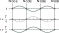
\includegraphics[scale=0.98]{figures/ch_14/fig_14_10.pdf}
			\caption[]{}
			\label{fig:14_10}
		\end{center}
	\end{minipage}
	\hfill{ }%space{-0.05cm}
	\begin{minipage}[t]{0.48\linewidth}
		\begin{center}
			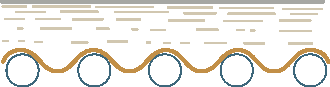
\includegraphics[scale=0.98]{figures/ch_14/fig_14_11.pdf}
			\caption[]{}
			\label{fig:14_11}
		\end{center}
	\end{minipage}
\vspace{-0.4cm}
\end{figure}

Differentiating \eqn{14_54} once with respect to $t$ and once with respect to $x$, we find expressions for the velocity of the particles $\dot{\xi}$ and the deformation of the medium $\varepsilon$:
\begin{align}
	\dot{\xi} &= \diff{\xi}{t} = - 2 \omega A \cos\parenthesis{ \frac{2\pi x}{\lambda} } \sin(\omega t), \label{eq:14_58}\\
	\varepsilon &= \diff{\xi}{x} = - 2 \frac{2\pi}{\lambda} A \sin\parenthesis{ \frac{2\pi x}{\lambda} } \cos(\omega t). \label{eq:14_59}
\end{align}

\noindent
Equation \eqref{eq:14_58} describes a standing wave of velocity, and \eqn{14_59} one of deformation.

Figure \ref{fig:14_11} compares ``instantaneous photographs'' of the displacement, velocity, and deformation for the time moments $0$ and $T/4$. Inspection of the graphs shows that the nodes and antinodes of the velocity coincide with their displacement counterparts; the nodes and antinodes of the deformation, however, coincide with the antinodes and nodes of the displacement, respectively.
When $\xi$ and $\varepsilon$ reach their maximum values, $\dot{\xi}$ becomes equal to zero, and vice versa.
Accordingly, the energy of a standing wave transforms twice during a period, once completely into potential energy mainly concentrated near the nodes of the wave (where the deformation antinodes are), and once completely into kinetic energy mainly concentrated near the antinodes of the wave (where the antinodes of the velocity are).
The result is the transition of energy from each node to its adjacent antinodes and back.
The time-averaged energy flux in any cross section of the wave is zero.

\section{Oscillations of a String}\label{sec:14_8}

When transverse oscillations are produced in a stretched string fastened at both ends, standing waves are set up in it, and there must be nodes at the places where the string is fastened.
Hence, only such oscillations are produced with an appreciable intensity in a string when the length of the latter is an integer multiple of half their wavelength (\fig{14_12}).
This gives the condition
\begin{equation}\label{eq:14_60}
	l = n \frac{\lambda}{2}\quad \text{or}\quad \ab{\lambda}{n} = \frac{2l}{n}\quad (n = 1, 2, 3, \ldots)
\end{equation}

\noindent
($l$ is the length of the string).
The following frequencies correspond to the wavelengths given by \eqn{14_60}:
\begin{equation}\label{eq:14_61}
	\ab{\nu}{n} = \frac{v}{\ab{\lambda}{n}} = \frac{v}{2l} n \quad (n = 1, 2, 3, \ldots)
\end{equation}

\noindent
($v$ is the phase velocity of the wave determined by the string tension and the mass per unit length, \ie, the linear density of the string).

The frequencies $\ab{\nu}{n}$ are called the \textbf{natural frequencies} of the string.
The natural frequencies are integral multiples of the frequency
\begin{equation*}
	\ab{\nu}{i} = \frac{v}{2l},
\end{equation*}

\noindent
called the \textbf{fundamental frequency}.

\begin{figure}[t]
	\begin{center}
		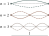
\includegraphics[scale=1]{figures/ch_14/fig_14_12.pdf}
		\caption[]{}
		\label{fig:14_12}
	\end{center}
	\vspace{-0.8cm}
\end{figure}

Harmonic oscillations with frequencies according to \eqn{14_61} are called \textbf{natural} or \textbf{normal oscillations}.
They are also known as \textbf{harmonics}.
In the general case, the oscillation of a string is a superposition of various harmonics.

The oscillations of a string are remarkable in the respect that according to classical notions, we get discrete values of one of the quantities characterizing the oscillations (their frequency).
Such a discrete nature is an exception for classical physics.
For quantum processes, it is the rule rather than an exception.

\section{Sound}\label{sec:14_9}

If elastic waves propagating in air have a frequency ranging from \SIrange{16}{20000}{\hertz}, then upon reaching the human ear, they cause a sound to be perceived.
Accordingly, elastic waves in any medium having a frequency confined within the above limits are called \textbf{sound waves} or simply \textbf{sound}.
Elastic waves with frequencies below \SI{16}{\hertz} are called \textbf{infrasound}, and those with frequencies above \SI{20000}{\hertz} are called \textbf{ultrasound}.
The human ear does not hear infra- and ultrasounds.

People distinguish sounds they hear by \textbf{pitch}, \textbf{timbre} (\textbf{quality}), and \textbf{loudness}.
A definite physical characteristic of a sound wave corresponds to each of these subjective appraisals.

Any real sound is not a simple harmonic oscillation, but is the superposition of harmonic oscillations with a definite set of frequencies.
The collection of frequencies of the oscillations present in a given sound is called its \textbf{acoustic spectrum}.
If a sound contains oscillations of all the frequencies within an interval from $\nu'$ to $\nu''$, then, the spectrum is called \textbf{continuous}.
If a sound consists of oscillations having the discrete frequencies $\nu_1$, $\nu_2$, $\nu_3$, etc., then, the spectrum is known as \textbf{a line one}.
Noises have a continuous acoustic spectrum.
Oscillations with a line spectrum produce the sensation of a sound with a more or less definite pitch.
Such a sound is called a \textbf{tone sound}, or simply a \textbf{tone}.

The pitch of a tone is determined by its fundamental (lowest) frequency.
The relative intensity of the \textbf{overtones} (\ie, of the oscillations of the frequencies $\nu_2$, $\nu_3$, etc.) determines the timbre, or quality, of the sound.
The different spectral composition of sounds produced by various musical instruments makes it possible to distinguish by ear, for example, a flute from a violin or a piano.

By the intensity of a sound is meant the time-averaged value of the density of the energy flux carried by a sound wave.
To be audible, a wave must have a certain minimum intensity known as the \textbf{threshold of hearing}.
This threshold differs somewhat for different persons and depends quite greatly on the frequency of the sound.
The human ear is most sensitive to frequencies from \SIrange{1000}{4000}{\hertz}.
In this region of frequencies, the threshold of hearing averages about \SI{e-12}{\watt\per\metre\squared}.
At other frequencies, it is higher (see the bottom curve in \fig{14_13}).

\begin{figure}[t]
	\begin{center}
		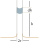
\includegraphics[scale=1]{figures/ch_14/fig_14_13.pdf}
		\caption[]{}
		\label{fig:14_13}
	\end{center}
	\vspace{-0.8cm}
\end{figure}

At intensities of the order of \SIrange{1}{10}{\watt\per\metre\squared}, a wave stops being perceived as a sound and produces only a feeling of pain and pressure in the ear.
The value of the intensity at which this occurs is known as the \textbf{threshold of pain} (or the \textbf{threshold of feeling}).
The pain threshold, like the hearing one, depends on the frequency (see the top curve in \fig{14_13}; the data given in this figure relate to the average normal hearing).

The subjectively estimated loudness of a sound grows much more slowly than the intensity of the sound waves.
When the intensity grows in a geometric progression, the loudness grows approximately in an arithmetical progression, \ie, linearly.
On these grounds, the \textbf{loudness level} $L$ is determined as the logarithm of the ratio between the intensity of the given sound $I$ and the intensity $I_0$ taken as the initial one:
\begin{equation}\label{eq:14_62}
	L = \log\parenthesis{\frac{I}{I_0}}.
\end{equation}

\noindent
The initial intensity $I_0$ is taken equal to \SI{e-12}{\watt\per\metre\squared} so that the hearing threshold at a frequency of the order of \SI{1000}{\hertz} is at the zero level ($L = 0$).

The unit of loudness level $L$ determined by \eqn{14_62} is called the \textbf{bell} (B).
Generally the \textbf{decibel} (\si{\decibel}), which is one-tenth of a bell is preferred.
The value of $L$ in decibels is determined by the equation
\begin{equation}\label{eq:14_63}
	L = 10 \log\parenthesis{\frac{I}{I_0}}.
\end{equation}

The ratio of two intensities $I_1$ and $I_2$ can also be expressed in decibels:
\begin{equation}\label{eq:14_64}
	L_{12} = 10 \log\parenthesis{\frac{I_1}{I_2}}.
\end{equation}

\noindent
This equation can be used to express the reduction in the intensity (the damping) of a wave over a certain path in decibels.
Thus, for example, a damping of \SI{20}{\decibel} signifies that the intensity has dropped to one-hundredth of its initial value.

The entire range of intensities at which a wave produces a feeling of sound in the human ear (from \SI{e-12}{\watt\per\metre\squared}), corresponds to values of the loudness level from \SIrange{0}{130}{\decibel}.
Table \ref{table:14_1} gives approximate values of the loudness level for selected sounds.

The energy which sound waves convey with them is extremely small.
If we assume, for example, that a glass of water completely absorbs the entire energy of a sound wave with a loudness level of \SI{70}{\decibel} falling on it (in this case the amount of energy absorbed per second will be about \SI{2e-7}{\watt}), then, to heat the water from room temperature to boiling about ten thousand years will be needed.

\begin{table}[!b]
	\renewcommand{\arraystretch}{1.2}
	\caption{}
	\vspace{-0.6cm}
	\label{table:14_1}
	\begin{center}\resizebox{0.65\linewidth}{!}{
			\begin{tabular}{lc}
				\toprule[1pt]
				\textbf{Sound} & \textbf{Loudness level}, \si{\decibel}\\
				\midrule[0.5pt]\midrule[0.5pt]
				Ticking of a clock & $20$\\
				Whisper at a distance of \SI{1}{\metre} & $30$\\
				Quiet conversation & $40$\\
				Speech of a moderate loudness & $60$\\
				Loud speech & $70$\\
				Shout & $80$\\
				Noise of an aircraft engine: &\\
				$\quad$ at a distance of \SI{5}{\metre} & $120$\\
				$\quad$ at a distance of \SI{3}{\metre} & $130$\\
				\bottomrule[1pt]
			\end{tabular}
	}\end{center}
\end{table}

Ultrasonic waves can be produced in the form of directed beams like beams of light.
Directed ultrasonic beams have found a widespread application for locating objects and determining the distance to them in water.
The first to put forward the idea of ultrasonic location was the outstanding French physicist Paul Langevin.
He implemented this idea during the first world war for detecting submarines.


At present, ultrasonic locators are used for detecting icebergs, fish shoals, and the like.

It is general knowledge that by shouting and determining the time that elapses until the echo arrives, \ie, the sound reflected by an obstacle---a mountain, forest, the surface of the water in a well, etc.---we can find the distance to the obstacle by multiplying half of this time by the speed of sound.
This principle underlies the locator (sonar) mentioned above, and also the ultrasonic echo sounder used to measure the depth and determine the relief of the sea bottom.

Ultrasonic location permits bats to orient themselves very well when flying in the dark.
A bat periodically emits pulses of an ultrasonic frequency and according to the reflected signals received by its ears assesses the distances to surrounding objects with a high accuracy.

\section{The Velocity of Sound in Gases}\label{sec:14_10}

A sound wave in a gas is a sequence of alternating regions of compression and rarefaction of the gas propagating in space.
Hence, the pressure at every point of space experiences a periodically changing deflection $\Delta{p}$ from its average value $p$ coinciding with the pressure existing in the gas when waves are
absent.
Thus, the instantaneous value of the pressure at a point of space can be written in the form
\begin{equation*}
	p' = p + \Delta{p}.
\end{equation*}

Assume that a wave is propagating along the $x$-axis.
Let us consider the volume of a gas in the form of a
cylinder with a base area of $S$ and an altitude of $\Delta{x}$ (\fig{14_14}), as we did in \sect{14_5} when finding the velocity of elastic waves in a solid medium.
The mass of the gas confined in this volume is $\rho S\Delta{x}$, where $\rho$ is the density of the gas undisturbed by the wave.
Owing to the smallness of $\Delta{x}$, the projection of the acceleration onto the $x$-axis
for all the points of the cylinder may be considered the same and equal to $\diffnpartialin{\xi}{t}2$.

\begin{figure}[t]
	\begin{center}
		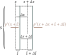
\includegraphics[scale=1]{figures/ch_14/fig_14_14.pdf}
		\caption[]{}
		\label{fig:14_14}
	\end{center}
	\vspace{-0.8cm}
\end{figure}

To find the projection onto the $x$-axis of the force exerted on the volume being considered, we must take the product of the cylinder base area $S$ and the difference between the pressures in the cross sections $(x+\xi)$ and $(x + \Delta{x} + \xi + \Delta{\xi})$.
Repeating the reasoning that led us to \eqn{14_34}, we get
\begin{equation*}
	F_x = - \diffpartial{p'}{x} S \Delta{x}
\end{equation*}

\noindent
[we remind our reader that when deriving \eqn{14_34} we took advantage of the assumption $\Delta{\xi}\ll\Delta{x}$].

Thus, we have found the mass of the separated volume of gas, its acceleration, and the force exerted on it.
Now let us write the equation of Newton's second law for this volume of gas:
\begin{equation*}
	(\rho S \Delta{x}) \diffnpartial{\xi}{t}{2} = - \diffpartial{p'}{x} S \Delta{x}.
\end{equation*}

\noindent
After cancelling $S\Delta{x}$, we get
\begin{equation}\label{eq:14_65}
	\rho \diffnpartial{\xi}{t}{2} = - \diffpartial{p'}{x}.
\end{equation}

The differential equation we have obtained contains two unknown functions, namely, $\xi$ and $p'$.
Let us express one of them through the other.
To do this, we shall find the relation between the pressure of a gas and the relative change in its volume $\diffpartialin{\xi}{x}$.
This relation depends on the nature of the process of compression (or rarefaction) of the gas.
The compressions and rarefactions of a gas in a sound wave follow one another so frequently that adjacent portions of the medium do not manage to exchange heat, and the process can be considered as an adiabatic one.
In an adiabatic process, the pressure and volume of a given mass of a gas are related by the equation
\begin{equation}\label{eq:14_66}
	p V^{\gamma} = \text{constant},
\end{equation}

\noindent
where $\gamma$ is the ratio between the heat capacities of the gas at constant pressure and at constant volume [see Eq. (10.42) of Vol. I].

In accordance with \eqn{14_66}:
\begin{equation*}
	p (S \Delta{x})^{\gamma} = p'[S(\Delta{x}+\Delta{\xi})]^{\gamma} = p' \bracket{ S \parenthesis{\Delta{x} + \diffpartial{\xi}{x} \Delta{x}} }^{\gamma} = p' (S \Delta{x})^{\gamma} \parenthesis{1+ \diffpartial{\xi}{x}}^{\gamma}.
\end{equation*}

\noindent
Cancelling $(S \Delta{x})^{\gamma}$ yeilds:
\begin{equation*}
	p = p' \parenthesis{1+ \diffpartial{\xi}{x}}^{\gamma}.
\end{equation*}

\noindent
Taking advantage of the assumption $\diffpartialin{\xi}{x}\ll 1$, let us expand the expression $\parenthesis{1+ \diffpartialin{\xi}{x}}^{\gamma}$ into a series by powers of $\diffpartialin{\xi}{x}$ and disregard the terms of the higher orders of smallness.
The result is
\begin{equation*}
	p = p' \parenthesis{ 1 + \gamma \diffpartial{\xi}{x} }.
\end{equation*}

\noindent
Let us solve this equation with respect to $p'$:
\begin{equation}\label{eq:14_67}
	p' = \frac{p}{\parenthesis{1 + \gamma \diffpartial{\xi}{x}}} \approx p \parenthesis{ 1 - \gamma \diffpartial{\xi}{x} }
\end{equation}

\noindent
[we have used the formula $1/(1+x)\approx 1-x$ holding for $x\ll 1$].
It is a simple matter to obtain an expression for $\Delta{p}$ from the relation we have found:
\begin{equation}\label{eq:14_68}
	\Delta{p} = p' - p = - \gamma p \diffpartial{\xi}{x}.
\end{equation}

Since the order of magnitude of $\gamma$ is near unity, it follows from \eqn{14_68} that $|\diffpartialin{\xi}{x}| \approx |\Delta{p}/p|$.
Thus, the condition, $\diffpartialin{\xi}{x}\ll 1$, signifies that the deviation of the pressure from its average value is much smaller than the pressure itself.
This is indeed true: for the loudest sounds, the amplitude of oscillations of the air pressure does not exceed \SI{1}{\mmHg}, whereas the atmospheric pressure $p$ has a value of the order of \SI{e3}{\mmHg}.

Differentiating \eqn{14_67} with respect to $x$, we find that
\begin{equation*}
	\diffpartial{p'}{x} = - \gamma p \diffnpartial{\xi}{x}{2}.
\end{equation*}

\noindent
Finally, using this value of $\diffpartialin{p'}{x}$ in \eqn{14_65}, we get the differential equation
\begin{equation*}
	\diffnpartial{\xi}{x}{2} = \frac{\rho}{\gamma p} \diffnpartial{\xi}{t}{2}.
\end{equation*}

\noindent
Comparing it with wave equation \eqref{eq:14_29}, we get the following expression for the velocity of sound waves in a gas:
\begin{equation}\label{eq:14_69}
	v = \parenthesis{\gamma \frac{p}{\rho}}^{1/2}
\end{equation}

\noindent
(we remind our reader that $p$ and $\rho$ are the pressure and the density of the gas undisturbed by a wave).

At atmospheric pressure and conventional temperatures, most gases are close in their properties to an ideal gas.
Therefore, we can assume that the ratio $p/\rho$ for them equals $RT/M$, where $R$ is the molar gas constant, $T$ is the absolute temperature, and $M$ is the mass of a mole of a gas [see Eq. (10.22) of Vol. I].
Introducing this value into \eqn{14_69}, we get the following equation for the velocity of sound in a gas:
\begin{equation}\label{eq:14_70}
	v = \parenthesis{ \frac{\gamma RT}{M}}^{1/2}.
\end{equation}

\noindent
Examination of this equation shows that the velocity of sound is proportional to the square root of the temperature and does not depend on the pressure.

The average velocity of thermal motion of gas molecules is determined by the formula
\begin{equation*}
	\average{\ab{v}{mol}} = \parenthesis{\frac{8RT}{\pi M}}^{1/2}
\end{equation*}

\noindent
[see Eq. (11.70) of Vol. I].
A comparison of this equation with \eqn{14_70} shows that the velocity of sound in a gas is related to the average velocity of thermal motion of its molecules by the expression
\begin{equation}\label{eq:14_71}
	v = \average{\ab{v}{mol}} \parenthesis{\frac{\gamma\pi}{8}}^{1/2}.
\end{equation}

\noindent
Substitution for $\gamma$ of its value for air equal to $1.4$ yields the expression $v\approx 3\average{\ab{v}{mol}}/4$.
The maximum possible value of $\gamma$ is $5/3$.
In this case, $v\approx 4\average{\ab{v}{mol}}/5$.
Thus, the velocity of sound in a gas is of the same order of magnitude as the average velocity of thermal motion of the molecules, but is always somewhat lower than $\average{\ab{v}{mol}}$.

Let us calculate the value of the velocity of sound in air at a temperature of \SI{290}{\kelvin} (room temperature).
For air, we have $\gamma=1.40$, and $M=\SI{29e-3}{\kilo\gram\per\mole}$.
The molar gas constant is $R=\SI{8.31}{\joule\per\mole\per\kelvin}$.
Introducing these values into \eqn{14_70}, we get
\begin{equation*}
	v = \parenthesis{\frac{\gamma RT}{M}}^{1/2} = \parenthesis{\frac{1.4\times 8.31 \times 290}{\num{29e-3}}}^{1/2} = \SI{340}{\metre\per\second}.
\end{equation*}

\noindent
The value of the sound velocity in air which we have found agrees quite well with the value found experimentally.

Let us find the relation between the intensity of a sound wave $I$ and the amplitude of the pressure oscillations $\ab{(\Delta{p})}{m}$.
We mentioned in \sect{14_9} that by the intensity of sound is meant the average value of the density of the energy flux.
Hence,
\begin{equation}\label{eq:14_72}
	I = \frac{1}{2} \rho A^2 \omega^2 v
\end{equation}

\noindent
[see \eqn{14_48}].
Here, $p$ is the density of the undisturbed gas, $A$ is the amplitude of oscillations of the particles of the medium, \ie, the amplitude of the oscillations of the displacement $\xi$, $\omega$ is the frequency, and $v$ the phase velocity of the wave.
We must note that in the given case the particles of the medium are understood to be macroscopic (\ie, including a great number of molecules) volumes, and not molecules; the linear dimensions of these volumes are much smaller than the wavelength.

Assume that $\xi$ changes according to the law $\xi=A\cos(\omega t-kx+\alpha)$.
Hence,
\begin{equation*}
	\diffpartial{\xi}{x} = Ak \sin(\omega t - k x + \alpha) = A \frac{\omega}{v} \sin(\omega t - k x + \alpha).
\end{equation*}

\noindent
Introducing this value into \eqn{14_68}, we obtain
\begin{equation*}
	\Delta{p} = - \gamma p A \frac{\omega}{v} \sin(\omega t - kx + \alpha) = - \ab{(\Delta{p})}{m} \sin(\omega t - kx + \alpha),
\end{equation*}

\noindent
whence
\begin{equation}\label{eq:14_73}
	A = \frac{\ab{(\Delta{p})}{m} v^2}{\gamma p \omega}.
\end{equation}

\noindent
Using this expression in \eqn{14_72}, we get
\begin{equation*}
	I = \frac{1}{2} \rho \frac{\ab{(\Delta{p})^2}{m} v^2}{\gamma^2 p^2 \omega^2} \omega^2 v = \frac{\ab{(\Delta{p})^2}{m}}{2 \gamma^2 \rho v} \parenthesis{\frac{\rho}{p}}^2 v^4.
\end{equation*}

\noindent
Taking into account that $v^4 = (\gamma RT/M)^2$, and $(p/\rho)^2 = (RT/M)^2$ [see \eqn{14_70} and the text preceding it], we can write that
\begin{equation}\label{eq:14_74}
	I = \frac{\ab{(\Delta{p})^2}{m}}{2 \rho v}.
\end{equation}

\noindent
We can use this equation to calculate the approximate values of the amplitude of air pressure oscillations corresponding to the range of loudness levels from \SIrange{0}{130}{\decibel}.
These values range from \SI{3e-5}{\pascal} (\SI{2e-7}{\mmHg}) to \SI{100}{\pascal} (about \SI{1}{\mmHg}).

Let us assess the amplitude of oscillations of the particles $A$ and that of the velocity of the particles $\ab{(\dot{\xi})}{m}$.
We shall begin with an assessment of the quantity $A$ determined by \eqn{14_73}.
Taking into account that $v/\omega=\lambda/(2\pi)$, we get the expression
\begin{equation}\label{eq:14_75}
	\frac{A}{\lambda} = \frac{1}{2\pi\gamma} \frac{\ab{(\Delta{p})^2}{m}}{p} \approx 0.1 \frac{\ab{(\Delta{p})^2}{m}}{p}
\end{equation}

\noindent
($\gamma\approx 1.5$, consequently, $2\pi\gamma\approx 10$).
At a loudness of \SI{130}{\decibel}, the ratio $\ab{(\Delta{p})^2}{m}/p$ has a value of the order of \num{e-3}, while at a loudness of \SI{60}{\decibel} this ratio is about \num{2e-7}.
The lengths of sound waves in air range from \SI{21}{\metre} (at $\nu = \SI{16}{\hertz}$) to \SI{17}{\milli\metre} (at $\nu = \SI{20000}{\hertz}$).
Inserting these values into \eqn{14_75}, we find that at a loudness of \SI{60}{\decibel} the amplitude of oscillations of the particles is about \SI{4e-4}{\milli\metre} for the longest waves and about \SI{3e-7}{\milli\metre} for the shortest ones.
At a loudness of \SI{130}{\decibel}, the amplitude of oscillations for the longest waves is about \SI{2}{\milli\metre}.

For harmonic oscillations, the amplitude of the velocity $\ab{(\dot{\xi})}{m}$ equals that of the displacement $A$ multiplied by the cyclic frequency $\omega$: $\ab{(\dot{\xi})}{m} = A\omega$.
Multiplying \eqn{14_75} by $\omega$, we get
\begin{equation}\label{eq:14_76}
	\frac{\ab{(\dot{\xi})}{m}}{v} = \frac{1}{\gamma} \frac{\ab{(\Delta{p})}{m}}{p} \approx \frac{\ab{(\Delta{p})}{m}}{p}.
\end{equation}

\noindent
Consequently, at a loudness of \SI{130}{\decibel}, the amplitude of the velocity is about $\SI{340}{\metre\per\second}\times\num{e-3}=\SI{0.34}{\metre\per\second}$.
At a loudness of \SI{60}{\decibel}, the amplitude of the velocity will be of the order of \SI{0.1}{\milli\metre\per\second}.
We must note that unlike the displacement amplitude, the velocity amplitude does not depend on the wavelength.

\section{The Doppler Effect for Sound Waves}\label{sec:14_11}

Assume that a device sensing the oscillations of the medium, which we shall call a receiver, is placed in a fluid at a certain distance from the wave source.
If the source and the receiver of the waves are stationary relative to the medium in which the wave is propagating, then the frequency of the oscillations picked up by the receiver will equal the frequency $\nu_0$ of the oscillations of the source.
If the source or the receiver or both are moving relative to the medium, then the frequency $\nu$ picked up by the receiver may differ from $\nu_0$.
This phenomenon is called the \textbf{Doppler effect}. [It is named after the Austrian scientist Christian Doppler (1803-1853) who described the effect for light waves.]

Let us assume that the source and the receiver move along the straight line joining them.
We shall assume the velocity of the source $\ab{v}{s}$ to be positive if it moves toward the receiver and negative if it moves away from the receiver.
Similarly, we shall assume the velocity of the receiver $\ab{v}{r}$ to be positive if the latter moves toward the source and negative if it moves away from the source.

If the source is stationary and oscillates with the frequency $\nu_0$, then by the moment when the source will complete its $\nu_0$-th oscillation, the ``crest'' of the wave produced by the first oscillation will travel the path $v$ in the medium ($v$ is the velocity of propagation of the wave relative to the medium).
Hence, the $\nu_0$ ``crests'' and ``troughs'' of the wave produced by the source in one second will cover the length $v$.
If the source is moving relative to the medium with the velocity $\ab{v}{s}$, then at the moment when the source completes its $\nu_0$-th oscillation, the crest produced by the first oscillation will be at a distance of $v-\ab{v}{s}$ from the source (\fig{14_15}).
Hence, the length $v-\ab{v}{s}$, will contain $\nu_0$ crests and troughs of a wave, so that the wavelength will be
\begin{equation}\label{eq:14_77}
	\lambda = \frac{v - \ab{v}{s}}{\nu_0}.
\end{equation}

\begin{figure}[t]
	\begin{center}
		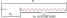
\includegraphics[scale=1]{figures/ch_14/fig_14_15.pdf}
		\caption[]{}
		\label{fig:14_15}
	\end{center}
	\vspace{-0.8cm}
\end{figure}

The stationary receiver will be passed in one second by the crests and troughs accommodated on the length $v$.
If the receiver is moving with the velocity $\ab{v}{r}$, then at the end of a time interval of one second it will pick up the trough which at the beginning of this interval was at a distance numerically equal to $v$ from its present position.
Thus, in one second, the receiver will pick up the oscillations corresponding to the crests and troughs accommodated on a length numerically equal to $v+\ab{v}{r}$ (\fig{14_16}) and will oscillate with the frequency
\begin{equation*}
	\nu = \frac{v + \ab{v}{r}}{\lambda}.
\end{equation*}

\noindent
Substituting for $\lambda$ its value from \eqn{14_77}, we get
\begin{equation}\label{eq:14_78}
	\nu = \nu_0 \parenthesis{\frac{v + \ab{v}{r}}{v - \ab{v}{s}}}.
\end{equation}

It follows from \eqn{14_78} that upon such motion of the source and the receiver when the distance between them diminishes, the frequency $\nu$ picked up by the receiver will be greater than that of the source $\nu_0$.
If the distance between the source and the receiver increases, $\nu$ will be less than $\nu_0$.

\begin{figure}[t]
	\begin{center}
		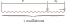
\includegraphics[scale=1]{figures/ch_14/fig_14_16.pdf}
		\caption[]{}
		\label{fig:14_16}
	\end{center}
	\vspace{-0.8cm}
\end{figure}

If the directions of the velocities $\ab{\vec{v}}{s}$ and $\ab{\vec{v}}{r}$ do not coincide with the straight line passing through the source and the receiver, then, the projections of the vectors $\ab{\vec{v}}{s}$ and $\ab{\vec{v}}{r}$ onto the direction of this straight line must be substituted for $\ab{v}{s}$ and $\ab{v}{s}$ in \eqn{14_78}.

Inspection of \eqn{14_78} shows that the Doppler effect for sound waves is determined by the velocities of the source and the receiver relative to the medium in which the sound propagates.
The Doppler effect is also observed for light waves, but the equation for the change in the frequency differs from \eqn{14_78}.
This is due to the fact that no material medium exists for light waves whose oscillations would be ``light''.
Therefore, the velocities of the source and the receiver of light relative to the ``medium'' are deprived of a meaning.
For light, we can speak only of the relative velocity of the receiver and the source.
The Doppler effect for light waves depends on the magnitude and direction of this velocity.
This effect will be considered for light waves in \sect{21_4}.
